\documentclass[10pt,twocolumn,letterpaper]{article}

\usepackage{cvpr}
\usepackage{times}
\usepackage{epsfig}
\usepackage{graphicx}
\usepackage{amsmath}
\usepackage{amssymb}

\usepackage{caption} 
\captionsetup[table]{skip=6pt}

\def\cvprPaperID{1} % *** Enter the CVPR Paper ID here

\usepackage[breaklinks=true,bookmarks=false]{hyperref}

\cvprfinalcopy % Comment this line and it stop working! :(
\ifcvprfinal\pagestyle{empty}\fi

\def\httilde{\mbox{\tt\raisebox{-.5ex}{\symbol{126}}}}

% Pages are numbered in submission mode, and unnumbered in camera-ready
%\ifcvprfinal\pagestyle{empty}\fi
\setcounter{page}{1}

\graphicspath{ {./images/} } 

\sloppy

%-------------------------------------------------------------------------
%-------------------------------------------------------------------------

\begin{document}

%%%%%%%%% TITLE
\title{Comparison of SegNet and U-Net for Semantic Segmentation}

\author{Felipe Augusto Lima Reis\\
PUC Minas - Pontif\'icia Universidade Cat\'olica de Minas Gerais\\
R. Walter Ianni 255 - Bloco L - Belo Horizonte, MG, Brasil\\
{\tt\small falreis@sga.pucminas.br}
}

\maketitle
%\thispagestyle{empty}

%%%%%%%%% ABSTRACT
%Briefly describe your problem, approach, and key results. Should be no more than 300 words.

\begin{abstract}
    Image segmentation refers to the partition of an image into a set of regions to cover it, to represent a meaningful area. Before the use of deep neural networks, the best-performing methods mostly was made using hand engineered features \cite{SEGNET}. This paper evaluates two Deep Neural Networks for semantic segmentation: SegNet and U-Net. These DNNs are both ``fully convolutional'' networks that output a result with the same size as the input. The goal of this paper is to compare the learning process of both networks with no pre or post processing to fit the dataset type of data. The models were trained and tested using KITTI Road Dataset. The results were evaluated using KITTI Dataset Toolkit. The tests showed that SegNet had a better performance in image segmentation than U-Net. SegNet was able to learn the dataset and ground truth information and predict with good accuracy. U-Net, however, was unable to learn the data information and pedict as expected, with unsatisfactory results.
\end{abstract}

%%%%%%%%% BODY TEXT


%##################################################################################################
\section{Introduction} \label{introduction}
%Describe the problem you are working on, why it's important, and an overview of your results

Image segmentation refers to the partition of an image into a set of regions to cover it, to represent meaningful areas \cite{DOMINGUEZ}. The goal is to simplify and/or change the representation of an image into something that is more meaningful and easier to analyze \cite{AHMED_SARMA}.

Segmentation has two main objectives: the first one is to decompose the image into parts for further analysis and the second one is to perform a change of representation \cite{DOMINGUEZ}. Also, segmentation must follow some characteristics to identify regions, as it follows:

\begin{itemize}
 \item Regions of an image segmentation should be uniform and homogeneous with respect to some characteristic, such as gray level, color, or texture \cite{DOMINGUEZ};
 \item Region interiors should be simple and without many small holes \cite{DOMINGUEZ};
 \item Adjacent regions of a segmentation should have significantly different values with respect to the characteristic on which they are uniform \cite{DOMINGUEZ};
 \item Boundaries of each segment should be smooth, not ragged, and should be spatially accurate \cite{DOMINGUEZ}.
\end{itemize}

Semantic pixel-wise segmentation is an active topic of research \cite{SEGNET}. Before the use of deep neural networks, the best-performing methods mostly was made using hand engineered features \cite{SEGNET}. The success of deep convolutional neural networks for object classification led researchers to use these techniques to learn new capabilities, such as segmentation \cite{SEGNET}.

This paper will evaluate two different Deep Neural Networks for semantic segmentation and compare the results over KITTI Road Dataset \cite{KITTI}. The chosen neural networks are SegNet \cite{SEGNET} and U-Net \cite{UNET}. The main goal of this work is to evaluate the networks with little training and without a post or a pre-processing transformation to increase the results to the dataset. Then, this paper did not apply any pre-processing or post-processing methods (except normalization) to increase the results over the dataset. Some transformations that can be pertinent to the dataset as bird-eye-view transformation, color-spacing changings, crop and some other transformation were not made to not influence the results.

The organization of this paper is as follows. In the next Section, we show related works to this paper. Section \ref{sec:data} contains information about the dataset used in this work as other datasets used previously to start the project. Section \ref{sec:methods} explains the methods used to develop this project, Section \ref{sec:experiments} describes the experiments and shows the results and Section \ref{sec:conclusion} concludes this paper and gives some final considerations and ideas for future works.


%##################################################################################################
\section{Related Work} \label{sec:related_work}
%Discuss published work that relates to your project. How is your approach similar or different from others?

Our approach follows the recent successes of deep neural networks for image classification \cite{VGGNET} \cite{AHMED_SARMA}, transfer learning \cite{PRATT} \cite{WEISS2016} and semantic segmentation \cite{SEGNET} \cite{UNET} \cite{FULLY_CONVOLU}. Also, the paper follows classical methods for segmentation \cite{WATERSHEDS} \cite{SLIC} \cite{LATTICES} \cite{FELZENSZWALB}, developed before the usage of neural nets.

\subsection{Superpixels} \label{ssec:superpixels}

Before the use of deep neural networks, the best-performing methods of segmentation mostly was made using hand engineered features \cite{SEGNET}. Some common features used pixels as basic units of processing \cite{WANG201728}. Superpixels are the result of perceptual grouping of pixels \cite{WANG201728}. Superpixels produces a segmentation of coarse granulation, that can be call over-segmentation \cite{WANG201728}. Superpixel segmentation showed to be a useful pre-processing step in many computer vision applications \cite{WANG201728}.

There has been a lot of research on superpixels since the term has been established \cite{WANG201728}. In particular, various algorithms for superpixel segmentations have been proposed. Algorithms for generating superpixels can be broadly categorized as either graph-based or gradient ascent methods \cite{SLIC}, as described below:

\begin{itemize}
 \item \textit{Graph-based algorithms}: Graph-based approaches to superpixel generation treat each pixel as a node in a graph. Edge weights between two nodes are proportional to the similarity between neighboring pixels. Superpixels are created by minimizing a cost function defined over the graph \cite{SLIC}. Example of this category is the \textit{Efficient Graph-Based Image Segmentation} (EGB) algorithm \cite{FELZENSZWALB} and the \textit{Superpixels Lattices} \cite{LATTICES};
 \item \textit{Gradient-ascent-based algorithms}: Starting from a rough initial clustering of pixels, gradient ascent methods iteratively refine the clusters until some convergence criterion is met to form superpixels \cite{SLIC}. In this set, it is possible to cite \textit{watersheds} algorithms \cite{WATERSHEDS} and the \textit{SLIC} algorithm \cite{SLIC};
\end{itemize}

%-------------------------------------------------------------------------
\subsection{Fully Convolutional Networks} \label{ssec:fully_conv}

Each layer of data in a Fully Convolutional Network (ConvNet) is a three-dimensional array of size $h \times w \times d$, where $h$ and $w$ are spatial dimensions, and $d$ is the feature or channel dimension \cite{FULLY_CONVOLU}. The first layer is the image, with pixel size $h \times w$, and $d$ color channels \cite{FULLY_CONVOLU}. Locations in higher layers correspond to the locations in the image they are path-connected to, which are called their receptive fields \cite{FULLY_CONVOLU}.

ConvNets are built on translation invariance. Their basic components (convolution, pooling, and activation functions) operate on local input regions and depend only on relative spatial coordinates \cite{FULLY_CONVOLU}. While a general deep net computes a general nonlinear function, a net with only layers of this form computes a
nonlinear filter, which we call a deep filter or fully convolutional network. An FCN naturally operates on an input of any size and produces an output of corresponding (possibly resampled) spatial dimensions \cite{FULLY_CONVOLU}.

%-------------------------------------------------------------------------
\subsubsection{SegNet} \label{sssec:segnet}

SegNet is a deep encoder-decoder architecture for multi-class pixel-wise segmentation \cite{SEGNET}. The SegNet architecture consists of a sequence of non-linear processing layers (encoders) and a corresponding set of decoders followed by a pixel-wise classifier \cite{SEGNET} \cite{SEGNET_WEBSITE}. In general, each encoder consists of one or more convolutional layers with batch normalization and a ReLU non-linearity, followed by non-overlapping max-pooling and sub-sampling \cite{SEGNET} \cite{SEGNET_WEBSITE}. The sparse encoding due to the pooling process is upsampled in the decoder using the max-pooling indices in the encoding sequence \cite{SEGNET} \cite{SEGNET_WEBSITE}. Figure \ref{fig:segnet} presents the architecture of SegNet.

\begin{figure}[ht]
  \centering
  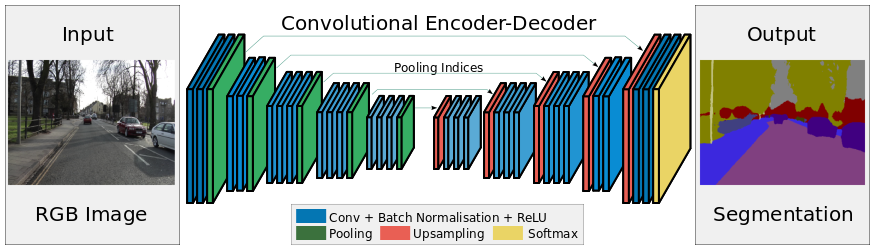
\includegraphics[width=0.48\textwidth]{segnet.png}
  \caption{SegNet architecture. \textit{Image adapted from SegNet project website} \cite{SEGNET_WEBSITE} \cite{SEGNET}}
  \label{fig:segnet}
\end{figure}

%-------------------------------------------------------------------------
\subsubsection{U-Net} \label{sssec:unet}

U-Net is a Convolutional Networks for Biomedical Image Segmentation \cite{UNET} \cite{UNET_WEBSITE}. Although U-Net was developed for biomedical image segmentation, its architecture can be trained to segment other types of image.

The U-Net architecture consists of the repeated application of two $3 \times 3$ convolutions, each followed by a rectified linear unit (ReLU) and a $2 \times 2$ max-pooling operation with stride 2 for downsampling \cite{UNET}. Every step in the expansive path consists of an up-sampling of the feature map followed by a $2 \times 2$ convolution, a concatenation with the correspondingly cropped feature map from the contracting path, and two $3 \times 3$ convolutions, each followed by a ReLU \cite{UNET}. At the final layer, a $1 \times 1$ convolution is used. In total the network has 23 convolutional layers \cite{UNET}. Figure \ref{fig:unet} presents the architecture of U-Net.

\begin{figure}[ht]
  \centering
  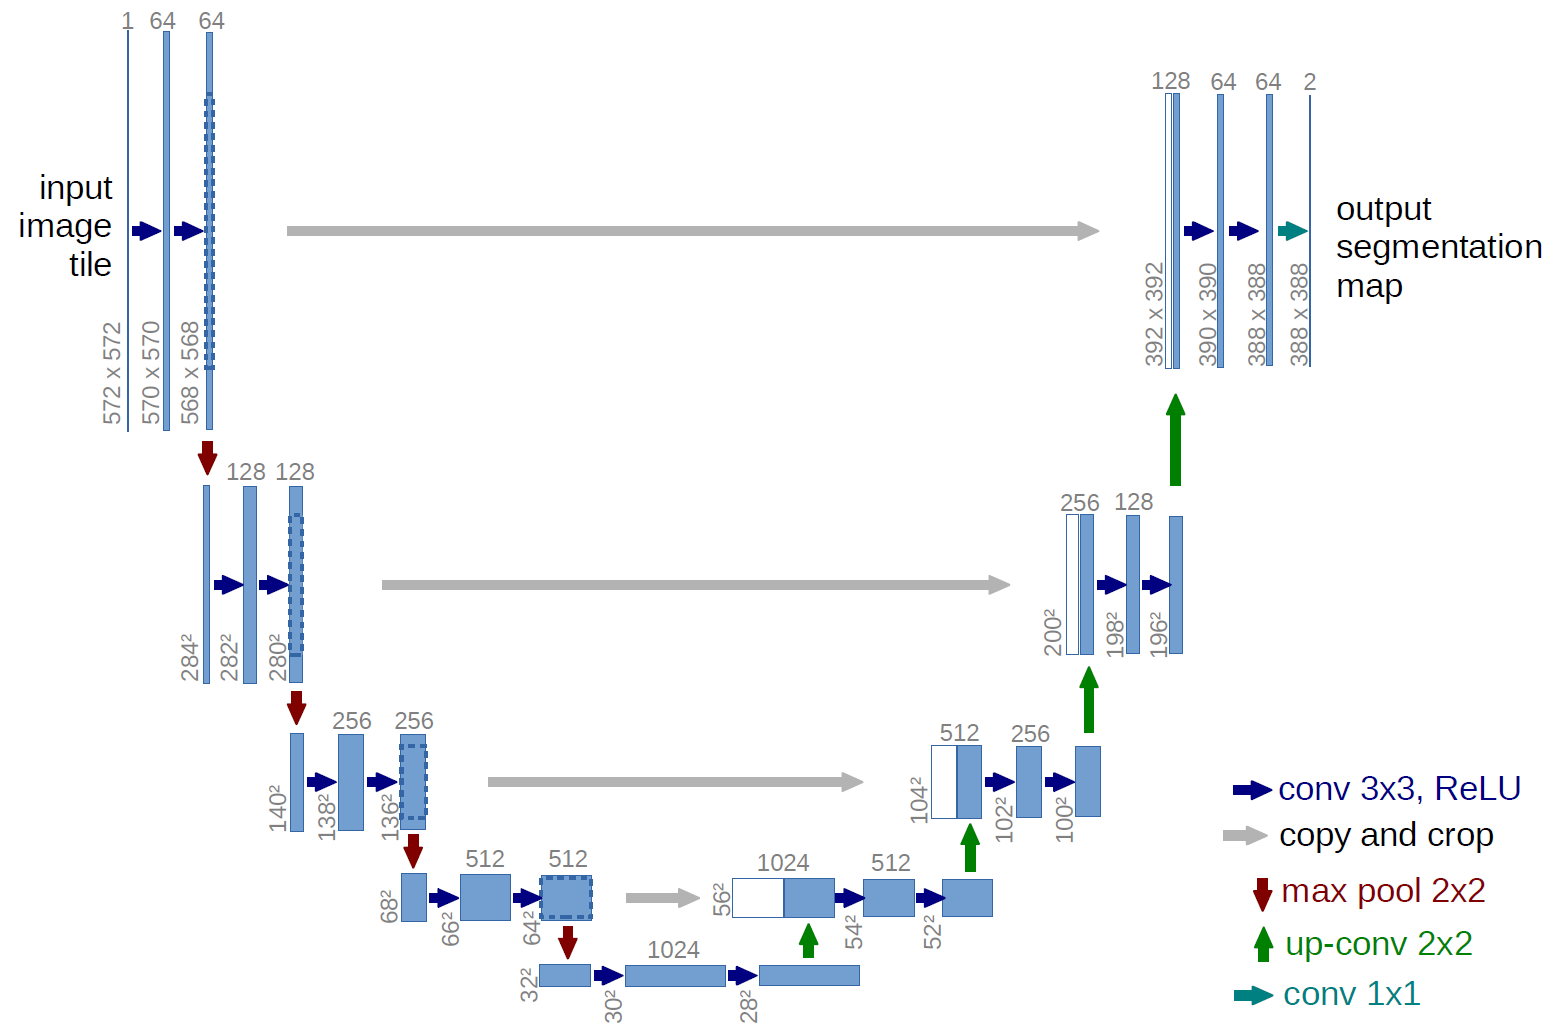
\includegraphics[width=0.48\textwidth]{unet.png}
  \caption{U-Net architecture. \textit{Image adapted from U-Net project website} \cite{UNET_WEBSITE} \cite{UNET}}
  \label{fig:unet}
\end{figure}


%##################################################################################################
\section{Data} \label{sec:data}

%Describe the data you are working with for your project. What type of data is it? Where did it come from? How much data are you working with? Did you have to do any preprocessing, filtering, or other special treatment to use this data in your project?

KITTI Vision Benchmarking Suite is a project of Karlsruhe Institute of Technology and Toyota Technological Institute at Chicago to provide a real-world computer vision benchmark for autonomous driving platform Annieway \cite{KITTI_FULL} \cite{KITTI_WEBSITE}. KITTI contains benchmarks and datasets for the following area of interests: stereo, optical flow, visual odometry, 3D object detection and 3D tracking \cite{KITTI_WEBSITE}.

One of the benchmarks in the KITTI suite is the Road/Lane Dataset Evaluation \cite{KITTI}. The road and lane estimation benchmark consists of 289 training and 290 test images, in four different categories of road scenes \cite{KITTI}:

\begin{itemize}
 \item uu - urban unmarked (98 training images and 100 test images) \cite{KITTI};
 \item um - urban marked (95 training images and 96 test images) \cite{KITTI};
 \item umm - urban multiple marked lanes (96 training images and 94 test images) \cite{KITTI};
 \item urban - combination of the three above \cite{KITTI}.
\end{itemize}

Ground truth has been generated by manual annotation of the images and is available for two different road terrain types: road - the road area (the composition of all lanes), and lane (the ego-lane, the lane the vehicle is currently driving on) \cite{KITTI} \cite{KITTI_WEBSITE}. Ground truth is provided for training images only \cite{KITTI}. 

As the dataset does not provide test ground truth, the results must be evaluated using a benchmarking tool provided with the dataset \cite{KITTI_WEBSITE}. This tool  performs road and lane estimation in the birds-eye-view space \cite{KITTI} \cite{KITTI_WEBSITE}. The metrics used are Maximum F1-measure, Average precision as used in PASCAL VOC challenges, Precision, Recall, False Positive Rate, False Negative Rate, F1 score and Hit Rate \cite{KITTI} \cite{KITTI_WEBSITE}.

%-------------------------------------------------------------------------
\subsection{Other Evaluated Datasets} \label{ssec:other_datasets}

The two datasets presented in this section were also evaluated for this paper, but, the final results do not contain both. The reasons to prefer KITTI over CamVid and BSDS500 datasets are available in Sections \ref{sec:experiments} and \ref{sec:conclusion}.

%-------------------------------------------------------------------------
\subsubsection{CamVid Dataset} \label{sssec:camvid_datasets}

The Cambridge-driving Labeled Video Database (CamVid) is the first collection of videos with object class semantic labels, complete with metadata \cite{CAMVID}. The database provides ground truth labels that associate each pixel with one of 32 semantic classes \cite{CAMVID}. The database addresses the need for experimental data to quantitatively evaluate emerging algorithms \cite{CAMVID}.

%-------------------------------------------------------------------------
\subsubsection{BSDS500 Dataset} \label{sssec:bsds_dataset}

Berkeley Segmentation Data Set contains 500 natural images and its respective ground-truths, annotated by humans \cite{BSDS500}. The images are explicitly separated into disjoint train, validation and test subsets \cite{BSDS500}.

To evaluate the quality of the segmentation methods, BSDS500 provides a benchmarking tool \cite{BSDS500}. BSDS500 dataset uses the Precision and Recall Method to evaluate the results \cite{BSDS500}.


%##################################################################################################
\section{Methods} \label{sec:methods}

%Discuss your approach for solving the problems that you set up in the introduction. Why is your approach the right thing to do? Did you consider alternative approaches? You should demonstrate that you have applied ideas and skills built up during the quarter to tackling your problem of choice. It may be helpful to include figures, diagrams, or tables to describe your method or compare it with other methods.

%-------------------------------------------------------------------------
\subsection{Data Augmentation} \label{ssec:data_augmentation}

Data augmentation consists of a range of transformations that can be applied to the dataset to increase the number of data with the target of improving the accuracy and robustness of classifiers \cite{AUGM_ADAPT}. The problem with small datasets is that models trained with them do not generalize well \cite{AUGM_DEEP}.

Data augmentation also can act as a regularizer in preventing overfitting in neural networks and improve performance in imbalanced class problems \cite{DATA_AUGM}. According to Wong et al. \cite{DATA_AUGM}, data augmentation is better to perform in data-space instead of feature-space, as long as label preserving transforms are known \cite{DATA_AUGM}.

To provide data augmentation, the training images and the respective ground-truth were flipped in the left-right direction, creating a ``mirror'' image. This procedure created 2 times more images to the training set, as shown in Image \ref{fig:data_augmentation}. 

\begin{figure}[ht]
  \centering
  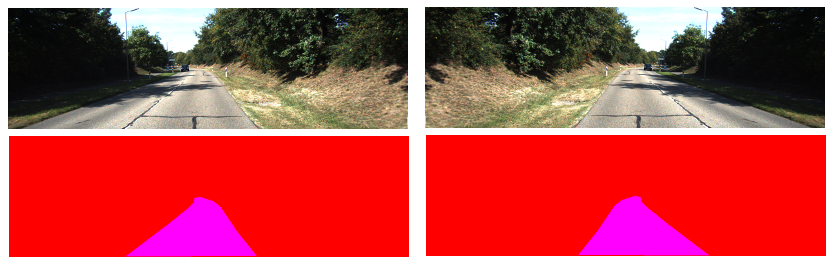
\includegraphics[width=0.48\textwidth]{data_augmentation.png}
  \caption{Data Augmentation with flip in left-right direction.}
  \label{fig:data_augmentation}
\end{figure}

One previous procedure applied to the data was a flip in an up-down direction, creating 3 more images than the original dataset. The results, however, were worse than with only left-right flip, more difficult to train and slower. The up-down data-augmentation, then, was removed.

%-------------------------------------------------------------------------
\subsection{Transfer Learning} \label{ssec:transfer_learning}

Transfer learning is a technique in machine learning that stores knowledge gained while solving one problem, adapt and apply it to a different but related problem. As the growth of neural networks usage, it becomes reasonable to seek out methods that avoid ``reinventing the wheel'', and instead are able to build on previously trained networks' results \cite{PRATT} \cite{WEISS2016}.

As the images of KITTI Dataset are really different from any other tested images, the use of transfer learning needs to shrink some parts of the image and grow other, deforming a lot the original image. Then, this work started trying to use transfer learning but decided to set aside the results.

%-------------------------------------------------------------------------
\subsection{Image Reduction} \label{ssec:image_reduction}

KITTI Road/Lane Dataset contains a three-dimensional image with the size of $375 \times 1242 \times 3$ (images size information for DNN was explained in Section \ref{ssec:fully_conv}). As the images were too big and to speed up the training process the images were reduced to the size of $ 184 \times 616 \times 3$. This size is almost half of the \textit{height} and \textit{width}. The size is not exactly half of the measures to keep SegNet and U-Net models with few changes, e.g. don't need to change the padding, kernel sizes, and other metrics, that can influence the tests.

%-------------------------------------------------------------------------
\subsection{Data Validation} \label{ssec:data_validation}

Once KITTI does not contain any validation data, a solution is to use part of the training data to validate the training procedure. To create that, the used procedure was split 20\% of the training set into a validation dataset. The training set was split using Keras Framework during the training period with shuffle mode ON.

%-------------------------------------------------------------------------
\subsection{Post Processing} \label{ssec:post_processing}

In this paper, no post-processing method was used to increase the results.

%-------------------------------------------------------------------------
\subsection{SegNet Model} \label{ssec:segnet_model}

SegNet model, as described in Section \ref{sssec:segnet}, uses the KITTI Lane/Road dataset images reduced to the size of $ 184 \times 616 \times 3$, as explained in Section \ref{ssec:image_reduction}. The SegNet model used in this project had the total of 5,468,890 parameters (5,464,270 trainable and 4,620 non-trainable). Table \ref{table:segnet_parameters} shows the number of parameters in each layer of SegNet architecture.

\begin{table}
  \scriptsize
  \begin{center}
  \begin{tabular}{{l}{l}{l}{l}}
  \hline 
    Num. & Layer (type) & Output Shape & Parameters \\
  \hline
    1	& Layer 1 		& (None, 3, 184, 616)	& 0	\\
    2	& Zero Padding 2D 	& (None, 3, 186, 618)	& 0 	\\
    3	& Convolution 2D 	& (None, 64, 184, 616)	& 1792	\\
    4	& Batch Normalization 	& (None, 64, 184, 616)	& 2464	\\
    5	& Activation		& (None, 64, 184, 616)	& 0 	\\
    6	& Max Pooling 2D	& (None, 64, 92, 308)	& 0     \\
    7	& Zero Padding 2D 	& (None, 64, 94, 310)	& 0 	\\
    8	& Convolution 2D 	& (None, 128, 92, 308)	& 73856	\\
    9	& Batch Normalization 	& (None, 128, 92, 308)	& 1232	\\
    10	& Activation		& (None, 128, 92, 308)	& 0 	\\
    11	& Max Pooling 2D	& (None, 128, 46, 154)	& 0 	\\
    12	& Zero Padding 2D 	& (None, 128, 48, 156)	& 0 	\\
    13	& Convolution 2D 	& (None, 256, 46, 154)	& 295168\\
    14	& Batch Normalization 	& (None, 256, 46, 154)	& 616	\\
    15	& Activation		& (None, 256, 46, 154)	& 0 	\\
    16	& Max Pooling 2D	& (None, 256, 23, 77)	& 0     \\
    17	& Zero Padding 2D 	& (None, 256, 25, 79)	& 0 	\\
    18	& Convolution 2D 	& (None, 512, 23, 77)	& 1180160\\
    19	& Batch Normalization 	& (None, 512, 23, 77)	& 308	\\
    20	& Activation		& (None, 512, 23, 77)	& 0 	\\
    21	& Zero Padding 2D 	& (None, 512, 25, 79)	& 0 	\\
    22	& Convolution 2D 	& (None, 512, 23, 77)	& 2359808\\
    23	& Batch Normalization 	& (None, 512, 23, 77)	& 308	\\
    24	& Up Sampling 2D	& (None, 512, 46, 154)	& 0	\\
    25	& Zero Padding 2D 	& (None, 512, 46, 154)	& 0 	\\
    26	& Convolution 2D 	& (None, 256, 46, 154)	& 1179904\\
    27	& Batch Normalization 	& (None, 256, 46, 154)	& 616	\\
    28	& Up Sampling 2D	& (None, 256, 92, 308)	& 0	\\
    29	& Zero Padding 2D 	& (None, 256, 94, 310)	& 0 	\\
    30	& Convolution 2D 	& (None, 128, 92, 308)	& 295040\\
    31	& Batch Normalization 	& (None, 128, 92, 308)	& 1232	\\
    32	& Up Sampling 2D	& (None, 128, 184, 616)	& 0	\\
    33	& Zero Padding 2D 	& (None, 128, 186, 618)	& 0 	\\
    34	& Convolution 2D 	& (None, 64, 184, 616)	& 73792	\\
    35	& Batch Normalization 	& (None, 64, 184, 616)	& 2464	\\
    36	& Convolution 2D 	& (None, 2, 184, 616)	& 130	\\
    37	& Reshape		& (None, 2, 113344)	& 0	\\
    38	& Permute		& (None, 113344, 2)	& 0	\\
    39	& Activation		& (None, 113344, 2)	& 0	\\
  \hline
    \multicolumn{4}{l}{Total params: 5,468,890} 	\\
    \multicolumn{4}{l}{Trainable params: 5,464,270}	\\
    \multicolumn{4}{l}{Non-trainable params: 4,620}	\\
  \hline
  \end{tabular}
  \caption{SegNet layers and its number of parameters}
  \label{table:segnet_parameters}
  \end{center}
\end{table}

As seen in Table \ref{table:segnet_parameters}, SegNet uses some techniques to improve the stability and performance of its network. One of the techniques is Batch Normalization, used to simplify models saturating nonlinearities, also called as internal covariate shift \cite{pmlr-v37-ioffe15}. Batch normalization consists in normalizing layer inputs for each training mini-batch \cite{pmlr-v37-ioffe15}. It allows the increase of learning rates and less careful parameter initialization \cite{pmlr-v37-ioffe15}. Batch normalization also acts as a regularizer, in some cases eliminating the need for Dropout \cite{pmlr-v37-ioffe15}. In the SegNet model, Batch Normalization was used 8 times with no usage of Dropout. 

One important feature that can be seen in Table \ref{table:segnet_parameters} is the distribution of the parameters across the network. Table \ref{table:segnet_parameters} shows that Convolution 2D layers contain the highest number of parameters to be trained, especially in the middle layers.

%-------------------------------------------------------------------------
\subsection{U-Net Model} \label{ssec:unet_model}

U-Net model, as described in Section \ref{sssec:unet}, uses the KITTI Lane/Road dataset images reduced to the size of $ 184 \times 616 \times 3$, as explained in Section \ref{ssec:image_reduction}. The U-Net model used in this project had the total of 471,586 parameters (all trainable). Table \ref{table:unet_parameters} shows the number of parameters in each layer of U-Net architecture.

\begin{table}
  \scriptsize
  \begin{center}
  \begin{tabular}{{l}{l}{l}{l}}
  \hline 
    Num. & Layer (type) & Output Shape & Parameters \\
  \hline
    1	& Layer 1 		& (None, 3, 184, 616)	& 0	\\
    2	& Convolution 2D 	& (None, 32, 184, 616)	& 896	\\
    3	& Dropout		& (None, 32, 184, 616)	& 0	\\
    4	& Convolution 2D 	& (None, 32, 184, 616)	& 9248	\\
    5	& Max Pooling 2D	& (None, 32, 92, 308)	& 0     \\
    6	& Convolution 2D 	& (None, 64, 92, 308)	& 18496	\\
    7	& Dropout		& (None, 64, 92, 308)	& 0	\\
    8	& Convolution 2D 	& (None, 64, 92, 308)	& 36928	\\
    9	& Max Pooling 2D	& (None, 64, 46, 154)	& 0     \\
    10	& Convolution 2D 	& (None, 128, 46, 154)	& 73856	\\
    11	& Dropout		& (None, 128, 46, 154)	& 0	\\
    12	& Convolution 2D 	& (None, 128, 46, 154)	& 147584\\
    13	& Up Sampling 2D 	& (None, 128, 92, 308)	& 0	\\
    14	& Concatenate (8+13)	& (None, 192, 92, 308)	& 0	\\
    15	& Convolution 2D 	& (None, 64, 92, 308)	& 110656\\
    16	& Dropout		& (None, 64, 92, 308)	& 0	\\
    17	& Convolution 2D 	& (None, 64, 92, 308)	& 36928	\\
    18	& Up Sampling 2D 	& (None, 64, 184, 616)	& 0	\\
    19	& Concatenate (4+18)	& (None, 96, 184, 616)	& 0	\\
    20	& Convolution 2D 	& (None, 32, 184, 616)	& 27680	\\
    21	& Dropout		& (None, 32, 184, 616)	& 0	\\
    22	& Convolution 2D 	& (None, 32, 184, 616)	& 9248	\\
    23	& Convolution 2D 	& (None, 2, 184, 616)	& 9248	\\
    24	& Reshape		& (None, 2, 113344)	& 0	\\
    25	& Permute		& (None, 113344, 2)	& 0	\\
    26	& Activation		& (None, 113344, 2)	& 0	\\
  \hline
    \multicolumn{4}{l}{Total params: 471,586} 	\\
    \multicolumn{4}{l}{Trainable params: 471,586}\\
    \multicolumn{4}{l}{Non-trainable params: 0}	\\
  \hline
  \end{tabular}
  \caption{U-Net layers and its number of parameters}
  \label{table:unet_parameters}
  \end{center}
\end{table}

As seen in Table \ref{table:unet_parameters}, U-Net does not contain Batch Normalization layers as SegNet. To improve stability and performance, U-Net uses Dropout Layers, a simple mechanism to avoid overfitting \cite{DROPOUT}. Also, Dropout does not contain parameters, reducing the total number of training parameters.

As SegNet, U-Net's Convolution 2D layers contain the highest number of parameters to be trained, especially in the middle layers, as seen in Table \ref{table:unet_parameters}.

One of important layer of U-Net, as seen in Table \ref{table:unet_parameters}, is the Merge/Concatenate Layers. The merge layer allows to create branches in the network. The input is passed to each sub layer and then the output of each layer is concatenated to form the output of the merged layers \cite{MERGE_WEBSITE}. Concatenate layers in U-NET merge two different branches in two different levels of the architecture.

%##################################################################################################
\section{Experiments} \label{sec:experiments}

%Discuss the experiments that you performed to demonstrate that your approach solves the problem. The exact experiments will vary depending on the project, but you might compare with previously published methods, perform an ablation study to determine the impact of various components of your system, experiment with different hyperparameters or architectural choices, use visualization techniques to gain insight into how your model works, discuss common failure modes of your model, etc. You should include graphs, tables, or other figures to illustrate your experimental results.

%-------------------------------------------------------------------------
\subsection{Environment} \label{ssec:environment}

The tests described in this section were performed in Amazon AWS \cite{AMAZON_WEBSITE} \textit{g2.2xlarge} instance running in North California data center. The instance contains 8 vCPUs of Intel Xeon E5-2670 CPU and 15GB RAM memory. Also, contains an NVIDIA Corporation GK104GL [GRID K520] GPU, with 4096 MB x2 GDDR5 memory. The custom configuration were a 100GB SSD storage capacity with a pre-configured Amazon Linux OS (Deep Learning AMI Version 12.0 - \textit{ami-f6a94495}).

The software environment used Python 3.5 \cite{PYTHON_WEBSITE} language, with Keras 2.2 \cite{KERAS}, a Python Deep Learning Library. Keras is a high-level neural networks API of running on top of TensorFlow \cite{TENSORFLOW}, CNTK \cite{CNTK}, or Theano \cite{THEANO} \cite{KERAS}. In this work, Keras run over Theano \cite{THEANO} backend. The virtual environment was provided by Anaconda \cite{ANACONDA_WEBSITE}. All environment requirements are available in a single file in the author's page project in Github \footnote{https://github.com/falreis/segmentation-eval/blob/master/code/i2dl.yml}.

For KITTI evaluation compatibility a new environment was created. KITTI needs Python 2.7, and older versions of NumPy and OpenCV libraries. The Anaconda environment requirement is available also in the author's page project in Github \footnote{https://github.com/falreis/segmentation-eval/blob/master/eval/kitti.yml}.

%-------------------------------------------------------------------------
\subsection{KITTI Road/Lane Experiments} \label{ssec:kitti_experiments}

To train SegNet and U-Net for KITTI dataset firstly was made preprocessing steps, e.g. data augmentation and image reduction, as explained in Sections \ref{ssec:data_augmentation} and \ref{ssec:image_reduction}. After these steps, the images were trained in Keras+Theano Environment and the best training weights were saved. Image \ref{fig:training_time} shows the average training time for each neural network. As predicted due the size of the neural net and the number of parameters to be trained, U-Net had a smaller training time than SegNet.

\begin{figure}[ht]
  \centering
  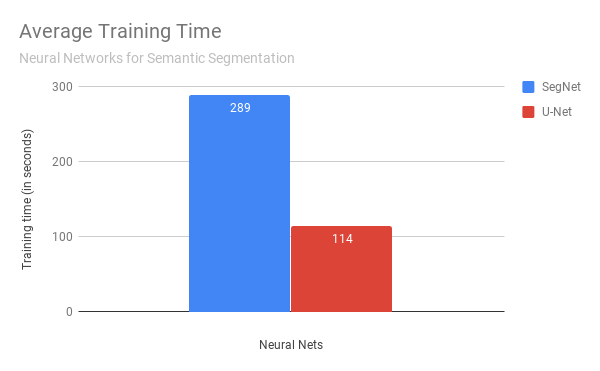
\includegraphics[width=0.48\textwidth]{graph_training_time.png}
  \caption{Time needed for training and validation step}
  \label{fig:training_time}
\end{figure}

The accuracy of the validation set (see \ref{ssec:data_validation}) for each neural network is visually represented in Image \ref{fig:val_acc}. The best value for SegNet was 86.87\% and for U-Net was 76.62\%. The loss on validation step is available in Image \ref{fig:val_loss}. The results show that SegNet performs better than U-Net at all times. In addition, the results show that U-Net easily reaches its best value. SegNet improves its results in the first few epochs and then the result floats near the best value.

\begin{figure}[ht]
  \centering
  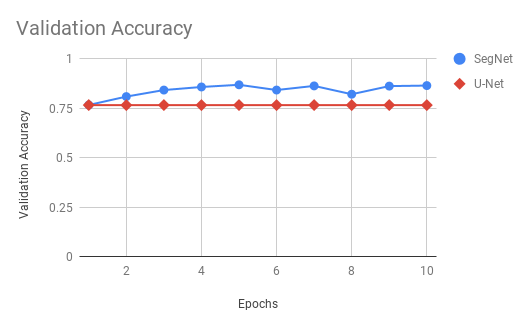
\includegraphics[width=0.48\textwidth]{graph_val_acc.png}
  \caption{Validation accuracy per epoch}
  \label{fig:val_acc}
\end{figure}

\begin{figure}[ht]
  \centering
  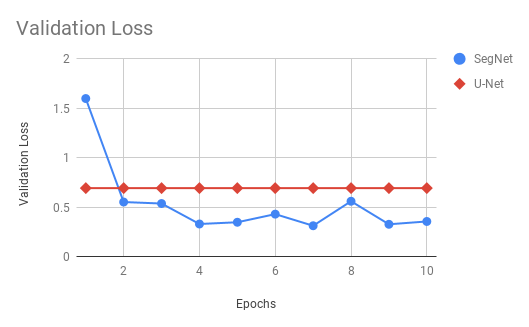
\includegraphics[width=0.48\textwidth]{graph_val_loss.png}
  \caption{Validation loss per epoch}
  \label{fig:val_loss}
\end{figure}

As seen in Figures \ref{fig:val_acc} and \ref{fig:val_loss}, U-Net reaches its best value and no longer improves. In the tests, many changes were made to increase the results such as the number of epochs, optimizer method and its values, and learning rate. In addition, the results were almost the same for the two data augmentation tested in this work (as explained in Section \ref{ssec:data_augmentation}).

After the training step, the best neural network achieved was used to predict the lane/road in the test images. The results of SegNet and U-Net for a test image is available in Image 
\ref{fig:neural_net_predict}.

\begin{figure}[ht]
  \centering
  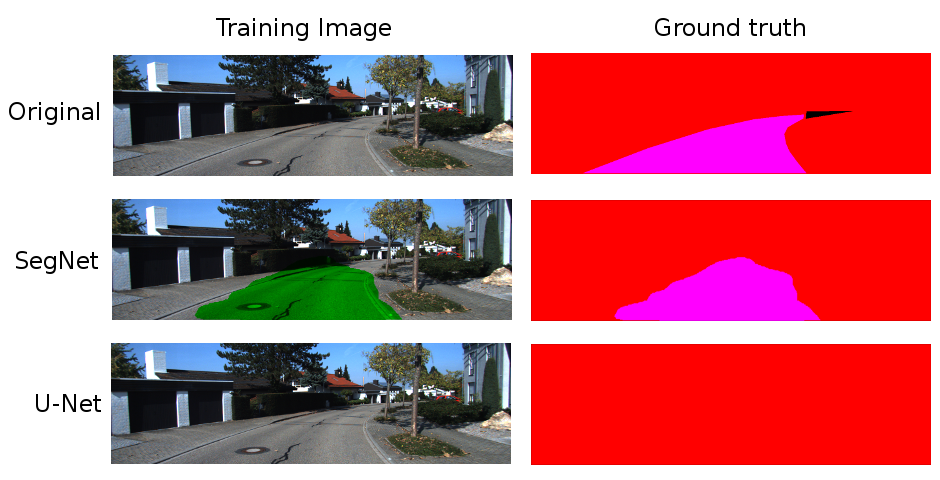
\includegraphics[width=0.48\textwidth]{comparison_nets.png}
  \caption{Comparison of SegNet and U-Net predictions for an image of the training set \textit{(uu\_000094.png)}.}
  \label{fig:neural_net_predict}
\end{figure} 

As seen in image \ref{fig:neural_net_predict}, the results predicted by SegNet were not very accurate. The results could be improved with other transformations to help the network to generalize, but it doesn't achieve the goal of this work.

As seen in Image \ref{fig:neural_net_predict}, the road was only predicted by SegNet neural network. U-Net just predicts a blank image, without marking the road. In an empirical test, it was observed that SegNet only starts to predict the road with poor precision when the validation accuracy was over 80\%. In the first epoch, SegNet didn't predict any road, as U-Net, which the best value was 76.62\%.

To evaluate the efficiency of the SegNet, it was used the KITTI evaluation benchmarking, as explained in Section \ref{sec:data}. The results were performed only in training set for 3 data categories and are available in Table \ref{table:kitti_eval}.

\renewcommand{\arraystretch}{1.3}%
\begin{table*}
  \captionsetup{justification=centering}
  \begin{center}
  \begin{tabular*}{0.62\linewidth}{{c}{c}{c}{c}{c}{c}{c}}
  \hline 	
    Category & MaxF & AP & PRE & REC & FPR & FNR \\
  \hline
    \textit{um\_lane} & 64.90\% & 44.84\% & 48.51\% & 98.02\% & 9.26\% & 1.98\% \\
    \textit{umm\_road} & 71.79\% & 62.91\% & 83.93\% & 62.72\% & 3.76\% & 37.28\% \\
    \textit{uu\_road} & 75.83\% & 62.14\% & 73.05\% & 78.84\% & 4.59\% & 21.16\% \\
  \hline
  \end{tabular*}
  \caption{KITTI benchmark evaluation results for SegNet in each category. \textit{MaxF: Maximum F1-measure, AP: Average precision, PRE: Precision, REC: Recall, FPR: False Positive Rate, FNR: False Negative Rate} \cite{KITTI_WEBSITE}}
  \label{table:kitti_eval}
  \end{center}
\end{table*}

Table \ref{table:kitti_eval} shows the best result for F-measure is 75.83\%. This results is good to identify the road but have a lot of noise. The result is well below the best algorithm available listed in the KITTI Road Dataset (96.60\%) \cite{KITTI_WEBSITE}.

%-------------------------------------------------------------------------
\subsection{Other Dataset Experiments} \label{ssec:other_experiments}

CamVid and BSDS500 datasets was briefly tested with SegNet neural network. 

The tests using CamVid dataset were performed just to test the code and compare the results with Observer07's Github repository\footnote{https://github.com/0bserver07/Keras-SegNet-Basic}, that contains the same test with CamVid set. CamVid tests was just performed few epochs and the results was not stored.

The BSDS500 data set was tested by SegNet, but the network did not provide good results. Because the BSDS500 dataset has only border images, the training set failed to generalize and produce a correct prediction. The validation set had more than 95\% accuracy at all steps, but only produced black images. Because most pixels are black in the BSDS500 data set, the neural network only predicted black pixels for each step with high accuracy. A possible solution to avoid this situation in a future work is to give weights to pixels. Black pixels should receive small values, while edge pixels (white) should receive large weights. This step could allow the neural network to increase the border pixel rate, instead of generalizing only the background of the image

%-------------------------------------------------------------------------
\subsection{Superpixel pre-processing Experiments} \label{ssec:superpixel_experiments}

In this paper, it was also performed some SLIC superpixels pre-processing experiments using KITTI dataset to verify the possible increase of performance of this method in U-Net and SegNet networks. The training images were divided into ~2048 superpixels (the exact number of superpixel can change due to SLIC algorithm behavior) and were recolored with the average pixel color, as seen in \ref{fig:kitt_superpixels}. 

\begin{figure}[ht]
  \centering
  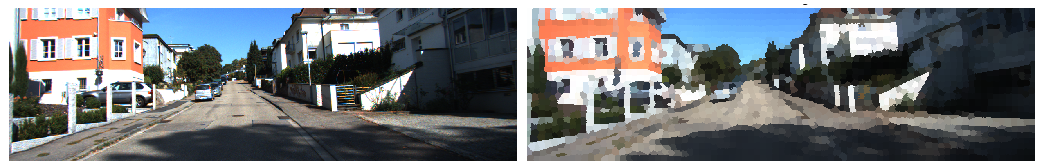
\includegraphics[width=0.48\textwidth]{kitti_superpixels.png}
  \caption{A training image \textit{(left)} and the result of SLIC algorithm with average pixel color recoloring \textit{(right)}}
  \label{fig:kitt_superpixels}
\end{figure} 

The superpixel preprocessing test had the main objective of trying to increase U-Net's performance, but superpixel recoloration did not result in any performance enhancements

%##################################################################################################
\section{Conclusion} \label{sec:conclusion}

%Summarize your key results - what have you learned? Suggest ideas for future extensions or new applications of your ideas.

Semantic pixel-wise segmentation is an important and active topic of research \cite{SEGNET}, and the usage of neural network is a trend in this area. The project compares the use of two famous Deep Neural Networks for semantic segmentation in a dataset different from that originally proposed for networks. Moreover, since the data were almost not preprocessed, this project could evaluate the robustness of the neural networks and the application in a different problem.

The results showed that SegNet can be used to solve problems of semantic segmentation in self-driving cars context with a relative accuracy with little pre and post-processing steps. In future works, it could be tested in different datasets to evaluate its capacity. U-Net, however, couldn't predict the results and didn't identify the road/lane properly. The usage of U-Net must be tested with transfer learning to and different parameters and techniques to verify if it can produce semantic segmentation results in this problem.

The tests performed in this works also shows that the number of parameters are very large, even with image size reduction. U-Net, despite having fewer parameters, failed to reach the network goal. Also, this paper shows that the number of layers, and the types of layers, can contribute in the learning process of semantic segmentation. One possible topic to study is the evaluation of the minimum size of network for semantic segmentation and the corresponding capacity to identify group of pixels.

As future work, its possible to compare other networks, like FCN-8, FCN-16, FCN-32 \cite{FULLY_CONVOLU} and some adapted VGG Nets \cite{VGGNET} to semantic segmentation. Also, it's possible to test different datasets in order to verify the adaptability of neural networks to different scenarios that its projected for. Also as future work, its possible to adapt different networks for boundaries segmentation, as briefly explained in Section \ref{ssec:other_experiments}.

%##################################################################################################
\section{Acknowledgements} \label{sec:acknowledgements}

This paper acknowledges some Github repositories that were helpful to provide some basic codes used in this work. This work started as a fork of \textit{divamgupta's} \textit{``image-segmentation-keras''} repository\footnote{https://github.com/divamgupta/image-segmentation-keras}. After a while, it used some code of \textit{Observer07's} \textit{``Keras-SegNet-Basic''} repository\footnote{https://github.com/0bserver07/Keras-SegNet-Basic}. Finally, the code changed a lot from both repositories and a new repository was created, \textit{``segmentation-eval''}\footnote{https://github.com/falreis/segmentation-eval}, with the code used to create this paper.

{\small
\bibliographystyle{ieee}
\bibliography{egbib}
}

\end{document}
